%!TEX root=../../root.tex

\section{Lezione 11}
\subsection{Problema appartenenza per CFG}
Dato $G = (V, \Sigma, R, S)$ e $w \in \Sigma^{\star}$ vogliamo sapere se $w \in L(G)$. Sia $n = |w|$, se $G$ è in forma normale di Chomsky $w$ è derivabile in $2n-1$ passi, poiché abbiamo bisogno di $n-1$ passi per arrivare da $S$ a $A_1 \dots A_n$ e altri $n$ passi per arrivare da $A_1 ... A_n$ a $a_1 ... a_n$. Quindi dato che le le derivazioni di parole lunghe $n$ sono lunghe $2n-1$ passi possiamo cercare $w$ tra tutte le derivazioni lunghe $2n-1$ passi. 
---manca complessità---
\subsection{Automi a pila}
Gli \textit{automi a pila} o $PDA$ (\textit{Push Down Automata}) sono un'estensione del concetto di $NFA$ che ci permettono di esprimere i linguaggi espressi dalle CFG. Ciò che hanno di nuovo è una pila che fornisce la possibilità di memorizzare più informazioni e quindi effettuare scelte più complesse. Ciò consente agli automi di riconoscere alcuni linguaggi non regolari. La pila viene acceduta in cima, sia in lettura che in scrittura, è inizialmente vuota e ogni volta che si "toglie" un carattere dalla pila, l'informazione è persa, così come ogni volta che si "mette" un carattere nella pila, prima di potervi accedere bisogna leggere e togliere i caratteri impilati successivamente.
\paragraph{Definizione formale}
Un $PDA$ è una sestupla
\[A = (Q, \Sigma, \Gamma, \delta, q_0, F)\]
Dove:
\begin{itemize}
	\item $Q$ è l'insieme degli stati
	\item $\Sigma$ è l'alfabeto di input
	\item $\Gamma$ è l'alfabeto sulla pila (che può coincidere con l'alfabeto di input);
	\item $\delta$ è la funzione di transizione: 
	$$\delta : Q \times \Sigma_{\varepsilon} \times \Gamma_{\varepsilon} \to \mathcal{P} ( Q \times \Gamma_{\varepsilon} )$$ Ossia dato uno stato di partenza $q \in Q$, un carattere letto in input $a \in \Sigma_{\varepsilon}$ e il carattere da leggere in cima alla pila $b \in \Gamma_{\varepsilon}$ la funzione $\delta$ ci dice l'insieme di stati in cui transitare e il relativo carattere da scrivere al posto del carattere letto. Quindi $\delta(q,a,x) = {(p,y), (r,z)}$ significa che da $q$ dopo aver letto $a$ possiamo transitare o in $p$ sostituendo $y$ ad $x$ in cima alla pila oppure in $r$ sostituendo $z$ ad $x$ in cima alla pila. Se $a = \varepsilon$ siamo aggiungendo un elemento in cima alla pila. Se $y = \varepsilon$ allora stiamo eliminando $a$ dalla cima della pila
	\item $q_0$ è lo stato iniziale
	\item $F$ è l'insieme degli stati finali
\end{itemize}

\paragraph{Classe dei linguaggi riconosciuti dai $PDA$}
Definiamo la classe e dei linguaggi riconosciuti dai $PDA$ come:
$$L(PDA) = \{L | \exists A \in PDA \land L(A) = L\}$$
\paragraph{Configurazioni in PDA}
Come negli automi a stati finiti anche nei PDA esiste il concetto di configurazione, in questo caso è una tripla $(q, x, w)$ dove:
\begin{itemize}
 \item  $q$ è lo stato corrente
 \item $x$ è la parola in input da leggere
 \item e $w$ è il contenuto della pila (il carattere più a sinistra è quello in cima alla pila)
 \end{itemize}
 Definiamo la relazione binaria "\textit{porta a}" $\Rightarrow$ tra due configurazioni per indicare che dalla prima, con un passo di calcolo, l'automa passa alla seconda; siano:
 \begin{itemize}
 \item $q, p \in Q$ due stati
 \item $a \in \Sigma_{\varepsilon}$, $x \in \Sigma^{\star}$ un carattere e una stringa di input
 \item $A, B \in \Gamma_{\varepsilon}$ due caratteri di pila e $\alpha \in \Gamma^{\star}$ una stringa nella pila 
 \end{itemize}
 $$(q, ax, A\alpha) \Rightarrow (p, x, B\alpha) \text{ sse } (p,B) \in \delta(q, a, A)$$
 
 Se $A = \varepsilon$ allora viene effettuato il push di $B$. Se $B = \varepsilon$ allora viene effettuato un pop di $A$.

Possiamo definire la chiusura riflessiva e transitiva di questa relazione con $\Rightarrow^{\star}$ che ci consente di descrivere più passi di calcolo e tornerà utile per fornire una descrizione del linguaggio accettato dall'automa.
\paragraph{Esempi PDA}
\begin{description}
	\item \textit{Esempio 1:} Costruiamo $A \in PDA$ t.c. $L(A) =\{ a^nb^n | n \geq 0\}$.
	\begin{figure}[H]
	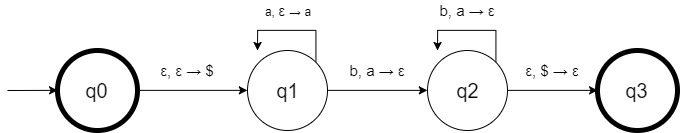
\includegraphics[scale=0.5]{p1}
	\end{figure}
	Diamo degli esempi di computazione:
	\begin{description}
		\item $(q_0, a^2b^2, \varepsilon) \Rightarrow (q_0, a^2b^2, \$) \Rightarrow (q_1, ab^2, a\$) \Rightarrow (q_1, b^2, a^2\$) \Rightarrow (q_2, b, a\$) \Rightarrow (q_2, \varepsilon, \$) \Rightarrow (q_3, \varepsilon, \varepsilon)$ \newline
	La parola viene correttamente accettata perché $q_3$ è finale e l'input è terminato. Notare che è ininfuente il fatto che la pila sia vuota ai fini dell'accettazione di una parola.
		\item $(q_0, a^4b^3, \varepsilon) \Rightarrow^{\star} (q_2, \varepsilon, a\$)$. La parola non viene accettata poiché $q_2$ non è finale.
		\item $(q_0, ab^2, \varepsilon) \Rightarrow^{\star} (q_3, b, \varepsilon)$. La parola non viene accettata poiché l'input non è stato completamente consumato.
	\end{description}
	\item \textit{Esempio 2:} Costruiamo $A \in PDA$ t.c. $L(A) =\{ a^nb^mc^{n-m} | n \geq m \geq 0\}$.
	\begin{figure}[H]
	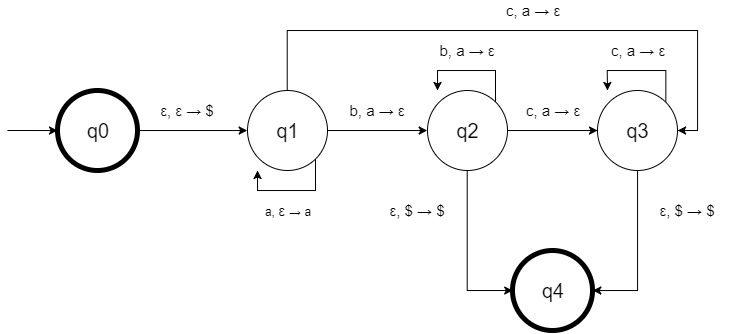
\includegraphics[scale=0.5]{p2}
	\end{figure}
	\item \textit{Esempio 3:} Costruiamo $A \in PDA$ t.c. $L(A) =\{ a^nb^{2n} | n \geq 0\}$.
	\begin{figure}[H]
	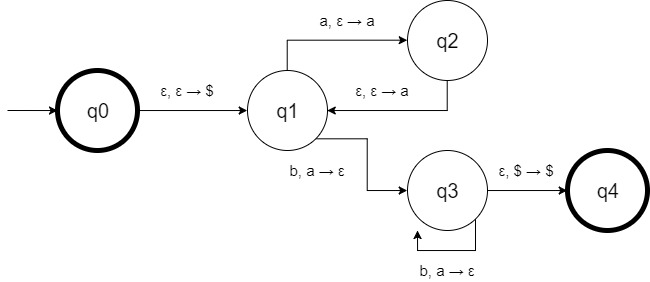
\includegraphics[scale=0.5]{p3}
	\end{figure}
\end{description}
\paragraph{Esercizi}
\begin{description}
	\item \textit{Esercizio 1:} Costruire $A \in PDA$ t.c. $L(A) =\{ a^nb^m | 0 \leq n \leq m \leq 2n \}$.
	\begin{figure}[H]
	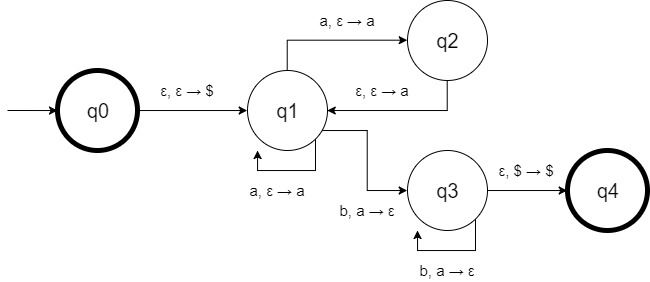
\includegraphics[scale=0.5]{p4}
	\end{figure}
	\item \textit{Esercizio 2:} Data la grammatica $G = ({S}, {0,1}, {S \to SS | 0S1 | 1S0 | \varepsilon}, S)$ fornire la descrizione del linguaggio che $G$ descrive.\newline
	\textit{Soluzione} $L = \{ x^n | n \geq 0 \land x \in \{0,1\}^{\star} \land n_1(x)=n_0(x)\}$, ossia un linguaggio formato da tutte parole che possono essere scomposte in sottostringhe tutte uguali in cui il numero di 1 è uguale al numero di 0.
	\item \textit{Esercizio 3:}  Data la grammatica $G = ({S, A}, {0,1}, {S \to AS | 0S1 | A, A \to 0A | 0 }, S)$ fornire la descrizione del linguaggio che $G$ descrive.\newline
	\textit{Soluzione:} $L = \{0^{n+k} 1^n | n \geq 0 \land k \geq 1\}$
	\item \textit{Esercizio 4:} Esprimere la grammatica dell'esercizio 2 in forma normale di Chomsky.\newline
	\textit{Soluzione:} Per essere sintetici scriveremo solo come vengono modificate le regole.
	\begin{enumerate}
		\setcounter{enumi}{0}
		\item \[S_0 \to S\] \[S \to SS | 0S1 | 1S0 | \varepsilon \]
		\item $NULL=\{S\}$
		\[S_0 \to S\] \[S \to SS | 0S1 | 01 | 1S0 | 10 \]
		\item $UNIT = \{(S_0, S_0),(S,S),(S_0, S)\}$
		\[S_0 \to  SS | 0S1 | 01 | 1S0 | 10 \] \[S \to SS | 0S1 | 01 | 1S0 | 10 \]
		\item $PROD = V$ e $DER = V$ quindi non dobbiamo fare modifiche.
		\item Aggiungiamo le regole per i terminali:
		\[A \to 0\]\[B \to 1\]
		\[S_0 \to  SS | ASB | AB | BSA | BA \] \[S \to SS | ASB | AB | BSA | BA \]
		Scomponiamo le regole in modo che la parte destra sia sempre di due variabili.
		\[A \to 0\]\[B \to 1\]\[C \to SB\]\[D \to SA\]
		\[S_0 \to  SS | AC | AB | BD | BA \] \[S \to SS |AC | AB | BD | BA \]
	\end{enumerate}
\end{description}
